Define the Hamiltonian in a second-quantized form and use this to compute the expectation value of the ground state (defining the so-called reference energy and later our Hartree-Fock functional) of
the helium atom.
Show that it is given by
\begin{equation}
    E[\Phi_0] = \expval{c}{\hat{H}}{c} = \sum_{i} \expval{i}{\hat{h}_0}{i} + \frac{1}{2} \sum_{ij} \left[\expval*{ij}{\frac{1}{r_{ij}}}{ij} - \expval*{ij}{\frac{1}{r_{ij}}}{ji}\right].
\end{equation}
Define properly the sums keeping in mind that the states $ij$ refer to all quantum numbers $n, l, m_l, s, m_s$.
Use the values for the various matrix elements listed at the end of the midterm to find the value of $E$ as function of $Z$ and compute $E$ as function of $Z$.

\subsection{}
We consider the Hamiltonian $\hat{H} = \hat{H}_0 + \hat{H}_I$, where $\hat{H}_0$ is the one-body part and $\hat{H}_I$ is the two-body part, given by
\begin{align*}
    \hat{H}_0 &= \sum_{i=1}^{N}\hat{h}_0(x_i), &
    \hat{H}_I &= \sum_{i<j}^{N}\frac{1}{r_{ij}}.
\end{align*}
In second quantization, we rewrite the one-body part as
\begin{equation}
    \hat{H}_0 = \sum_{\alpha\beta} \expval{\alpha}{\hat{h}_0}{\beta} a_\alpha^\dagger a_\beta.
\end{equation}
With the new annihilation and creation operators $b_\alpha$ and $b_\alpha^\dagger$ with respect to the new vacuum state $\ket*{\Phi_0}$, we can rewrite this as
\begin{equation}\label{eq:H0_second_quant}
    \begin{split}
        \hat{H}_0 =& \sum_{ab} \expval{a}{\hat{h}_0}{b} b_a^\dagger b_b + \sum_{ai} \left[ \expval{a}{\hat{h}_0}{i} b_a^\dagger b_i^\dagger + \expval{i}{\hat{h}_0}{a} b_i b_a \right] \\
        &+ \sum_{i} \expval{i}{\hat{h}_0}{i} - \sum_{ij} \expval{j}{\hat{h}_0}{i} b_i^\dagger b_j.
    \end{split}
\end{equation}

Recalling that
\begin{equation*}
    \expval{\alpha}{\hat{h}_0}{\beta} = -\frac{Z^2}{2n^2}\delta_{\alpha \beta},
\end{equation*}
we can simplify the expression to
\begin{equation*}
    \hat{H}_0 = \sum_{a} \expval{a}{\hat{h}_0}{a} b_a^\dagger b_a + \sum_{i} \expval{i}{\hat{h}_0}{i} - \sum_{i} \expval{i}{\hat{h}_0}{i} b_i^\dagger b_i.
\end{equation*}
The first and last terms vanish, as both $b_b \ket*{\Phi_0} = 0$ and $b_j \ket*{\Phi_0} = 0$, leaving us with
\begin{equation}
    \hat{H}_0 = \sum_{i} \expval{i}{\hat{h}_0}{i}.
\end{equation}

The two-body part is rewritten in second quantization as
\begin{equation}
    \hat{H}_I = \frac{1}{2} \sum_{\alpha \beta \gamma \delta} \expval{\alpha \beta}{V}{\gamma \delta} a_\alpha^\dagger a_\beta^\dagger a_\delta a_\gamma.
\end{equation}
With the new annihilation and creation operators, we can rewrite this as
\begin{equation*}
    \hat{H}_I = \hat{H}_I^{(1)} + \hat{H}_I^{(2)} + \hat{H}_I^{(3)} + \hat{H}_I^{(4)} + \hat{H}_I^{(5)},
\end{equation*}
where utilizing antisymmetrized matrix elements for the sake of brevity, we have
\begin{align*}
    \hat{H}_I^{(1)} &= \frac{1}{4} \sum_{abcd} \expval{ab}{V}{cd} b_a^\dagger b_b^\dagger b_d b_c, \\
    \hat{H}_I^{(2)} &= \frac{1}{4} \sum_{abci} \expval{ab}{V}{ci} b_a^\dagger b_b^\dagger b_i^\dagger b_c + \expval{ai}{V}{cb} b_a^\dagger b_i b_b b_c \\
    \hat{H}_I^{(3)} &= \frac{1}{4} \sum_{abij} \left[\expval{ab}{V}{ij} b_a^\dagger b_b^\dagger b_j^\dagger b_i^\dagger + \expval{ij}{V}{ab} b_a b_b b_j b_i \right] \\
    &\qquad + \frac{1}{2} \sum_{abij} \expval{ai}{V}{bj} b_a^\dagger b_j^\dagger b_b b_i + \frac{1}{2} \sum_{abi} \expval{ai}{V}{bi} b_a^\dagger b_b \\
    \hat{H}_I^{(4)} &= \frac{1}{4} \sum_{aijk} \left[ \expval{ai}{V}{jk} b_a^\dagger b_k^\dagger b_j^\dagger b_i + \expval{ji}{V}{ak} b_k^\dagger b_j b_i b_a \right] \\
    &\qquad + \frac{1}{2} \sum_{aij} \left[ \expval{ai}{V}{ji} b_a^\dagger b_j^\dagger + \expval{ji}{V}{ai} {\color{red} b_j b_a} - \expval{ji}{V}{ia} b_j b_a \right] \\
    \hat{H}_I^{(5)} &= \frac{1}{4} \sum_{ijkl} \expval{kl}{V}{ij} b_i^\dagger b_j^\dagger b_l b_k + \frac{1}{2} \sum_{ijk} \expval{ij}{V}{kj} b_k^\dagger b_i + \frac{1}{2} \sum_{ij} \expval{ij}{V}{ij}.
\end{align*}

In order to simplify the computations later, we briefly summarize the qualitative properties of each of the terms above.
\begin{enumerate}[(1).]
    \item Contributes for $\geq$two-particle states
    \item Creates or removes a three-particle-one-hole state, while conserving the number of particles
    \item Term by term,
        \begin{enumerate}
            \item Creates a two-particle-two-hole state by either removing two particles and creating two holes, or by removing two holes and creating two particles.
            \item Creates two one-particle-one-hole pairs.
            \item Contributions between particle pairs, and the hole states.
        \end{enumerate}
    \item Term by term,
        \begin{enumerate}
            \item Creation of a one-particle-one-hole pair, interacting with a hole.
            \item One-particle-one-hole pair interacting with a hole.
        \end{enumerate}
    \item Term by term,
        \begin{enumerate}
            \item Interactions between pairs of two hole states.
            \item Interactions between a hole and the other holes.
            \item Energy from the ground state.
        \end{enumerate}
\end{enumerate}

\begin{comment}
    In terms of the ground state, we only have contributions from the terms involving $b_{\alpha}^\dagger$.
    Everything else vanishes.
    \begin{enumerate}[(1.)]
        \item No contribution $b_c \ket*{\Phi_0} = 0$
        \item No contribution $b_c \ket*{\Phi_0} = 0$
        \item
            \begin{enumerate}[(a)]
                \item No contribution by orthogonality
                \item No contribution $b_i \ket*{\Phi_0} = 0$
                \item No contribution $b_b \ket*{\Phi_0} = 0$
            \end{enumerate}
        \item
            \begin{enumerate}[(a)]
                \item No contribution $b_i \ket*{\Phi_0} = 0$ and $b_a \ket*{\Phi_0} = 0$
                \item No contribution orthogonality, and lack of one-particle-one-hole states
            \end{enumerate}
        \item
            \begin{enumerate}
                \item
            \end{enumerate}
    \end{enumerate}
\end{comment}

We can now quickly see that $\expval{c}{\hat{H}_I}{c}$ only gets a contribution from the last $H_I^{(5)}$ term, as the other terms vanish due to either an annihilation operator acting on the vacuum state, or orthogonality of the states created.
We are then just left with
\begin{equation}
    \expval{\Phi_0}{\hat{H}_I}{\Phi_0} = \frac{1}{2} \sum_{ij} \expval{ij}{V}{ij}_{AS} = \frac{1}{2} \sum_{ij} \expval{ij}{V}{ij} - \expval{ij}{V}{ji}.
\end{equation}

Finally, combining this with the expectation value of the one-body part, we get that the complete expectation value of the ground state is
\begin{equation}
    E[\Phi_0]
    = \expval{c}{\hat{H}}{c}
    = \sum_{i} \expval{i}{\hat{h}_0}{i} + \frac{1}{2} \sum_{\substack{ij \\ i \neq j}} \left[\expval*{ij}{\frac{1}{r_{ij}}}{ij} - \expval*{ij}{\frac{1}{r_{ij}}}{ji}\right],
\end{equation}
as we wanted to show.

\begin{comment}
    Computing the results of $\expval{\Phi_0}{\hat{H}_I^{(5)}}{\Phi_0}$ term by term, we get the possible contractions
    \begin{equation*}
        \arraycolsep=1.4pt
        \begin{array}{ccrcccr}
            \langle \Phi_0 \vert
            \wick
            {
                \c2 b_i^\dagger
                \c1 b_j^\dagger
                \c1 b_l
                \c2 b_k
            }
            \vert \Phi_0 \rangle
            &=& \delta_{i k} \delta_{j l} &\implies& &&  \expval{i j}{V}{i j},  \\
            \langle \Phi_0 \vert
            \wick
            {
                \c1 b_i^\dagger
                \c2 b_j^\dagger
                \c1 b_l
                \c2 b_k
            }
            \vert \Phi_0 \rangle
            &=& -\delta_{i l} \delta_{j k} &\implies& -\expval{j i}{V}{i j} &= &-\expval{i j}{V}{j i}, \\
        \end{array}
    \end{equation*}
    from the first term.
    For the second we just get $\delta_{ik}$, giving us a term $\frac{1}{2} \sum_{ij} \expval{ij}{V}{ij}$.
    This leaves us with the expectation value of the two-body part as
    \begin{align*}
        \expval{\Phi_0}{\hat{H}_I}{\Phi_0} &= \expval{\Phi_0}{\hat{H}_I^{(5)}}{\Phi_0} \\
        &= \sum_{ij} \frac{1}{4} \left[ \expval{i j}{V}{i j} - \expval{i j}{V}{j i} \right] + \frac{1}{2} \sum_{ij} \expval{ij}{V}{ij} + \frac{1}{2} \sum_{ij} \expval{ij}{V}{ij} \\
    \end{align*}
\end{comment}
\begin{comment}
    \newpage

    Then, the expectation value of the ground state with the one-body part is given by
    \begin{equation*}
        \expval{\Phi_0}{\hat{H}_0}{\Phi_0} = \sum_{\alpha\beta} \expval{\alpha}{\hat{h}_0}{\beta} \expval{\Phi_0}{a_\alpha^\dagger a_\beta}{\Phi_0}.
    \end{equation*}
    For all states where either $\alpha > F, \beta > F$, we have that $\expval{\Phi_0}{a_\alpha^\dagger a_\beta}{\Phi_0} = 0$.
    Thus, the sum is restricted to $i,j \le F$,
    \begin{align*}
        \expval{\Phi_0}{\hat{H}_0}{\Phi_0} &= \sum_{ij} \expval{i}{\hat{h}_0}{j} \expval{\Phi_0}{a_i^\dagger a_j}{\Phi_0} \\
        &= \sum_{ij} \expval{i}{\hat{h}_0}{j} \delta_{ij} \\
        &= \sum_{i} \expval{i}{\hat{h}_0}{i},
    \end{align*}
    where we utilized the orthonormality of the single-particle states.

    The two-body part is rewritten in second quantization as
    \begin{equation*}
        \hat{H}_I = \frac{1}{2} \sum_{\alpha \beta \gamma \delta} \expval{\alpha \beta}{V}{\gamma \delta} a_\alpha^\dagger a_\beta^\dagger a_\delta a_\gamma.
    \end{equation*}
    The expectation value of the ground state with the two-body part is then
    \begin{equation*}
        \expval{\Phi_0}{\hat{H}_I}{\Phi_0} = \frac{1}{2} \sum_{\alpha\beta\gamma\delta} \expval{\alpha\beta}{V}{\gamma\delta} \expval{\Phi_0}{a_\alpha^\dagger a_\beta^\dagger a_\delta a_\gamma}{\Phi_0}.
    \end{equation*}
    The possible contributing contractions are
    \begin{align*}
        \wick{\c2 a_\alpha^\dagger \c1 a_\beta^\dagger \c1 a_\delta \c2 a_\gamma} &= \delta_{\alpha\gamma} \delta_{\beta\delta}, &
        \wick{\c1 a_\alpha^\dagger \c2 a_\beta^\dagger \c1 a_\delta \c2 a_\gamma} &= -\delta_{\alpha\delta} \delta_{\beta\gamma}. \\
    \end{align*}
    Whenever $\alpha > F$ or $\beta > F$, the expectation value vanishes, so we relabel the summation to $i, j$. The terms also vanish if $i = j$. % TODO: Reword maybe
    We are then left with
    \begin{equation*}
        \expval{\Phi_0}{\hat{H}_0}{\Phi_0} = \frac{1}{2} \sum_{\substack{ij \\ i \neq j}} \expval*{ij}{V}{ij} - \expval*{ij}{V}{ji}.
    \end{equation*}

    Gathering this, we get that the complete expectation value of the ground state is
    \begin{equation}
        E[\Phi_0]
        = \expval{c}{\hat{H}}{c}
        = \sum_{i} \expval{i}{\hat{h}_0}{i} + \frac{1}{2} \sum_{\substack{ij \\ i \neq j}} \expval*{ij}{\frac{1}{r_{ij}}}{ij} - \expval*{ij}{\frac{1}{r_{ij}}}{ji},
    \end{equation}
    as we wanted to show.
\end{comment}

In the case of the electrons in the helium atom, we only have $n = 1$, $l = 0$, differing only in the spin quantum number $m_s = \pm 1/2$.
The expectation value of the one-body part is then
\begin{equation*}
    \expval{\Phi_0}{\hat{h}_0}{\Phi_0} = \sum_{\sigma \in \{\pm 1/2\}} \expval{1\sigma}{\hat{h}_0}{1\sigma} = -\frac{Z^2}{n^2},
\end{equation*}
and the expectation value of the two-body part is, writing just $\sigma_{+}$ and $\sigma_{-}$ for the spins,
\begin{equation*}
    \expval{\Phi_0}{\hat{H}_I}{\Phi_0}
    = \frac{1}{2} \sum_{\substack{\sigma_{+}\sigma_{-}\\ \sigma_{+} \neq \sigma_{-}}}
    \underbrace{\expval*{\sigma_{+} \sigma_{-}}{\frac{1}{r_{\sigma_{+}\sigma_{-}}}}{\sigma_{+} \sigma_{-}}}_{\textnormal{Direct term}}
    - \underbrace{\expval*{\sigma_{+} \sigma_{-}}{\frac{1}{r_{\sigma_{+}\sigma_{-}}}}{\sigma_{-}\sigma_{+}}}_{\textnormal{Exchange term}}.
\end{equation*}
The exchange term vanishes since the states are orthogonal, and we are left with the direct term.
We are then just left with
\begin{equation*}
    \expval{\Phi_0}{\hat{H}_I}{\Phi_0} = \frac{1}{2}\left[ \expval*{\sigma_{+} \sigma_{-}}{\frac{1}{r_{\sigma_{+} \sigma_{-}}}}{\sigma_{+} \sigma_{-}} + \expval*{\sigma_{-} \sigma_{+}}{\frac{1}{r_{\sigma_{+} \sigma_{-}}}}{\sigma_{-} \sigma_{+}}\right].
\end{equation*}
As $\hat{H}_I$ is invariant under the change of label $\sigma$, we can simplify this to
\begin{equation*}
    \expval{\Phi_0}{\hat{H}_I}{\Phi_0} = \expval*{\sigma_{+} \sigma_{-}}{\frac{1}{r_{\sigma_{+} \sigma_{-}}}}{\sigma_{+} \sigma_{-}}.
\end{equation*}

Computing this, we find that the expectation value of the ground state is
\begin{equation}
    E[\Phi_0] = -Z^2 + \tfrac{5}{8}Z,
\end{equation}
which as a function of $Z$ is shown in \autoref{fig:energy}.

\begin{figure}[ht]
    \centering
    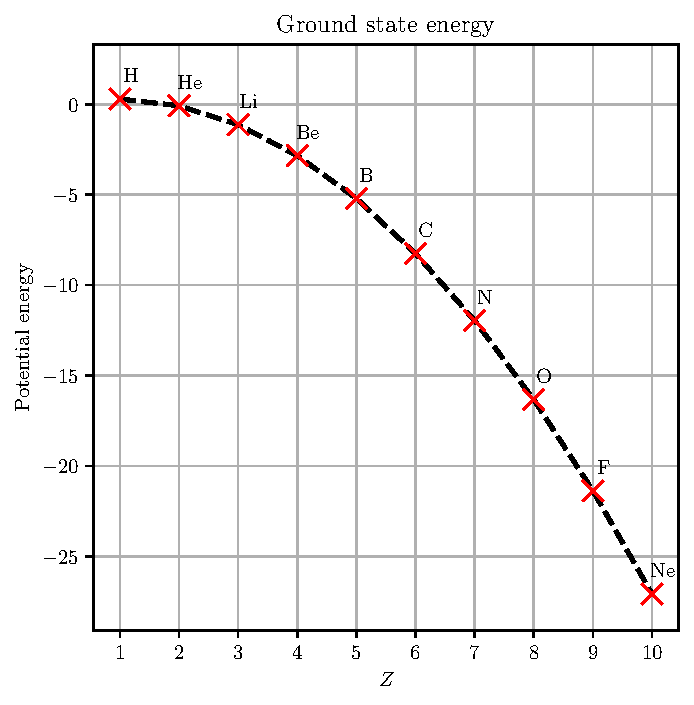
\includegraphics{figs/energy_plot.pdf}
    \caption{The expectation value of the ground states of an atom with two electrons as a function of the nuclear charge $Z$.\label{fig:energy}}
\end{figure}
